\documentclass[11pt,aspectratio=169]{beamer}

\usetheme{Singapore}
\usecolortheme{orchid}

\usepackage[utf8]{inputenc}
\usepackage[russian]{babel}
\usepackage{amsmath}
\usepackage{amsfonts}
\usepackage{amssymb}
\usepackage{graphicx}
\usepackage{bibentry}
\usepackage{wasysym}
\usepackage[most]{tcolorbox}
\usepackage[normalem]{ulem}

\usepackage{hyperref}

\definecolor{info}{RGB}{62, 180, 137}
\definecolor{warn}{RGB}{128, 0, 0}

\author{Николай Анохин}
\title{Метрики и базовые подходы}

\logo{
\includegraphics[width=.05\textwidth]{images/ok_logo.png}}

\AtBeginSection[]{
  \begin{frame}
  \vfill
  \centering
  \begin{beamercolorbox}[sep=8pt,center,shadow=true,rounded=true]{title}
    \usebeamerfont{title}\insertsectionhead\par
  \end{beamercolorbox}
  \vfill
  \end{frame}
}

%\setbeamercovered{transparent} 
%\setbeamertemplate{navigation symbols}{} 
%\logo{} 
%\institute{} 
%\date{} 
%\subject{} 

\begin{document}

{
\setbeamertemplate{headline}{}

\begin{frame}
\titlepage
\end{frame}

}

\begin{frame}{Контекст}

\begin{center}
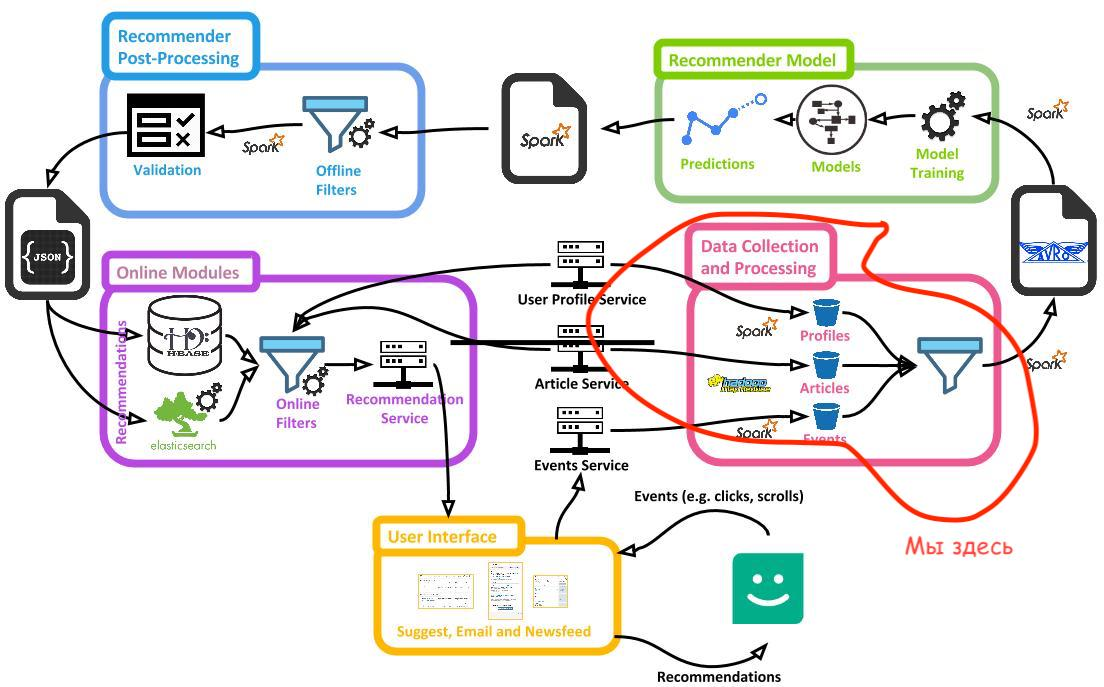
\includegraphics[scale=0.23]{images/mendeley.jpeg}
\end{center}

\end{frame}

\section{Оценка успешности идей}

\begin{frame}{Научный метод}

\begin{columns}
\begin{column}{0.45\textwidth}   
   \begin{center}
      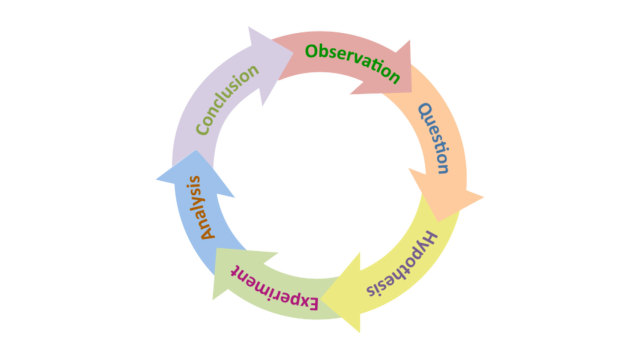
\includegraphics[scale=0.35]{images/method.jpeg}
    \end{center}
\end{column}
\begin{column}{0.45\textwidth}
    \begin{tcolorbox}[colback=gray!5,colframe=gray!80,title=]
       Чем быстрее проходим все этапы, тем быстрее улучшаем сервис
    \end{tcolorbox}
\end{column}
\end{columns}

\end{frame}

\begin{frame}{A/B эксперимент \cite{RSHB}}

\begin{columns}
\begin{column}{0.47\textwidth}
   \begin{tcolorbox}[colback=info!5,colframe=info!80,title=Плюсы]
      \begin{itemize}
      \item Надежная оценка эффекта на любую метрику
      \end{itemize}
    \end{tcolorbox}
\end{column}
\begin{column}{0.47\textwidth}
    \begin{tcolorbox}[colback=warn!5,colframe=warn!80,title=Минусы]
      \begin{itemize}
       \item Риск необратимо расстроить пользователей
       \item Риск финансовых потерь
       \item Дорого заводить
       \item Долго ждать результат
       \item Метрик не всегда достаточно
      \end{itemize}
    \end{tcolorbox}
\end{column}
\end{columns}

\end{frame}

\begin{frame}{}

\begin{tcolorbox}[colback=gray!5,colframe=gray!80,title=Миссия компании КнигаЛиц]
Helping users feel closer to their friends and family.
\end{tcolorbox}

\vfill

Q: Какую метрику вы бы предложили измерять в A/B?

\end{frame}

\begin{frame}{Опрос пользователей}

\begin{columns}
\begin{column}{0.47\textwidth}
   \begin{tcolorbox}[colback=info!5,colframe=info!80,title=Плюсы]
      \begin{itemize}
      \item Полный контроль над экспериментом
      \item Оценка эффекта на любую метрику
      \item Собрать фидбэк напрямую
      \end{itemize}
    \end{tcolorbox}
\end{column}
\begin{column}{0.47\textwidth}
    \begin{tcolorbox}[colback=warn!5,colframe=warn!80,title=Минусы]
      \begin{itemize}
       \item Дорогой сбор данных
       \item Смещение аудитории
       \item Нечестный фидбэк
      \end{itemize}
    \end{tcolorbox}
\end{column}
\end{columns}

\end{frame}

\begin{frame}{Офлайн эксперимент}

\begin{columns}
\begin{column}{0.47\textwidth}
   \begin{tcolorbox}[colback=info!5,colframe=info!80,title=Плюсы]
      \begin{itemize}
      \item Большая скорость проверки гипотез
      \item Нельзя сломать прод
      \end{itemize}
    \end{tcolorbox}
\end{column}
\begin{column}{0.47\textwidth}
    \begin{tcolorbox}[colback=warn!5,colframe=warn!80,title=Минусы]
      \begin{itemize}
       \item Не все метрики доступны офлайн
       \item Смещение выборки
       \item Результат не обязан обобщаться
      \end{itemize}
    \end{tcolorbox}
\end{column}
\end{columns}

\end{frame}

\section{Офлайн эксперимент}

\begin{frame}{Зачем улучшать RS}

\begin{footnotesize}

бизнесу
\begin{itemize}
\item Увеличить продажи
\item Продвигать более разнообразные айтемы
\item Улучшить пользовательский опыт
\item Добиться большей лояльности
\item Лучше понимать пользователей
\end{itemize}

пользователям
\begin{itemize}
\item Найти лучший товар
\item Найти {\bf все} подходящие товары
\item Найти последовательность или набор товаров
\item Залипнуть
\item Найти рекомендер, которому можно доверять
\item Реализовать творческие потребности
\item Помочь другим сделать выбор
\end{itemize}

\end{footnotesize}

\end{frame}

\begin{frame}{}

\begin{tcolorbox}[colback=gray!5,colframe=gray!80,title=Бизнесовая метрика]
напрямую интересует бизнес
\begin{itemize}
  \item сложно оптимизировать
  \item сложно понять, как компоненты системы влияют на метрику
  \item сложно мерить офлайн
 \end{itemize}
\end{tcolorbox}
\vfill
\begin{tcolorbox}[colback=gray!5,colframe=gray!80,title=Техническая метрика]
отражает один аспект системы
\begin{itemize}
  \item можно оптимизировать
  \item можно померить офлайн
  \item не интересует бизнес :(
 \end{itemize}
\end{tcolorbox}

\end{frame}

\begin{frame}{Какой бывает фидбэк}

\begin{columns}
\begin{column}{0.55\textwidth}
   \begin{center}
     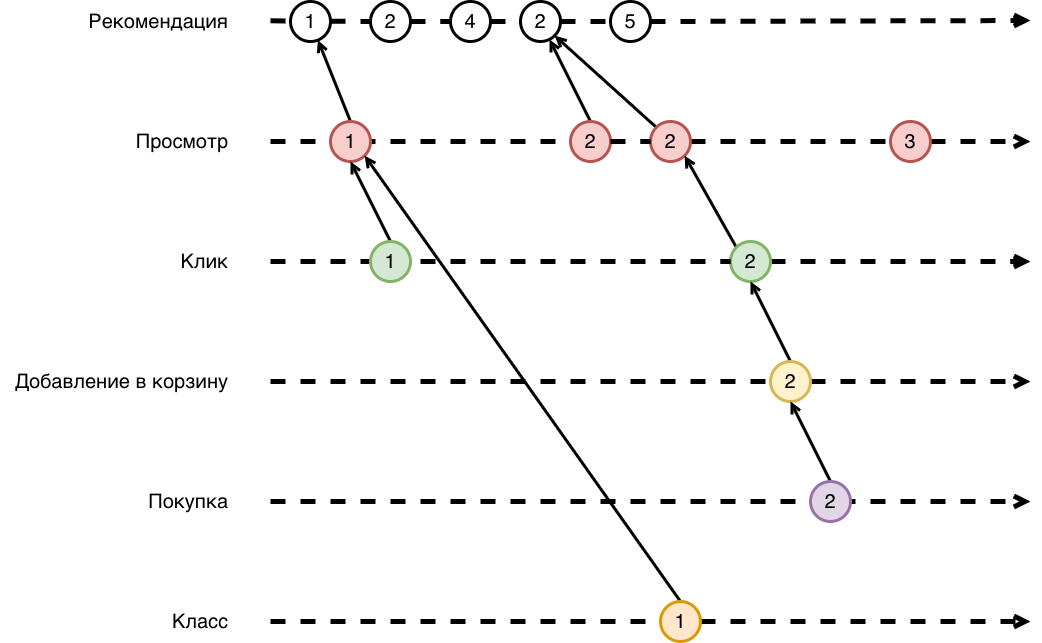
\includegraphics[scale=0.2]{images/recommendation-events.png}
  \end{center}
\end{column}
\begin{column}{0.4\textwidth}
    \begin{tcolorbox}[colback=gray!5,colframe=gray!80,title=Техническая метрика]
    \begin{itemize}%[<+->]
    \item[-] Явный/explicit
    \item[-] Неявный/implicit
    \item[-] Отложенный/delayed
    \end{itemize}
    \end{tcolorbox}
\end{column}
\end{columns}

\end{frame}

\begin{frame}{}

\begin{tcolorbox}[colback=info!5,colframe=info!80,title=]
При офлайн оценке нужно стремиться к тому, чтобы данные были максимально похожи на реальность
\end{tcolorbox}

\vfill

Техники выбора данных для офлайн оценки
\begin{itemize} %[<+->]
\item Семплировать случайные пары user-item
\item Семплировать случайные item у каждого пользователя 
\item Семплировать тестовых пользователей
\item Тестовые данные после обучающих по времени
\item Написать симулятор системы
\end{itemize}

\end{frame}

\section{Релевантность}

\begin{frame}{Pinkamena Diane Pie}

\begin{columns}
\begin{column}{0.4\textwidth}
   \begin{center}
		
\includegraphics[scale=0.25]{images/pony.jpeg}
   \end{center}
\end{column}
\begin{column}{0.55\textwidth}
    \begin{tcolorbox}[colback=info!5,colframe=info!80,title=]
    A comic relief character [...] appears to be the naive party animal of the group, she also displays admirable skill in science and engineering.
    \end{tcolorbox}
\end{column}
\end{columns}

\end{frame}

\begin{frame}{Релевантность}

\begin{tcolorbox}[colback=info!5,colframe=info!80,title=]
Насколько рекомендации соответствуют вкусам пользователя?
\end{tcolorbox}

\begin{center}
\includegraphics[scale=0.2]{images/relevance.png}
\end{center}

\end{frame}

\begin{frame}{Метрики точности}

\begin{center}
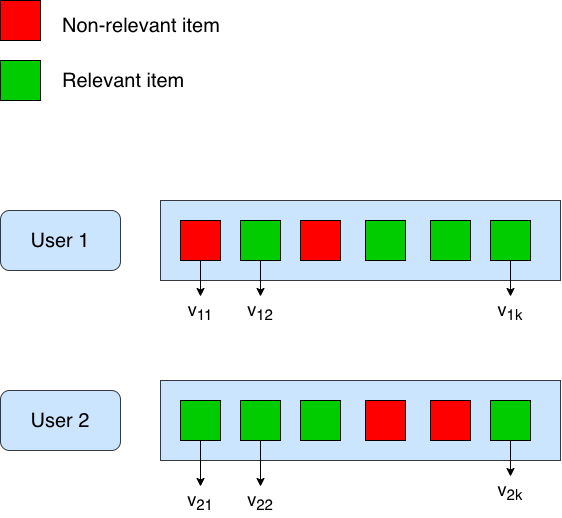
\includegraphics[scale=0.3]{images/pointwise-metrics.png}
\end{center}
RMSE, MAE, accuracy, precision, recall, auc, ...

\end{frame}

\begin{frame}{Метрики ранжирования}

\begin{center}
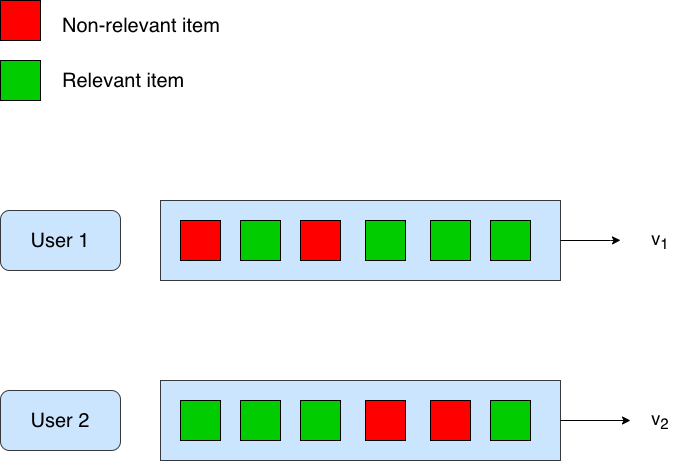
\includegraphics[scale=0.3]{images/ranking-metrics.png}
\end{center}

\end{frame}

\begin{frame}{Precision@k, Recall@k}

\begin{columns}
\begin{column}{0.5\textwidth}
   \begin{center}
		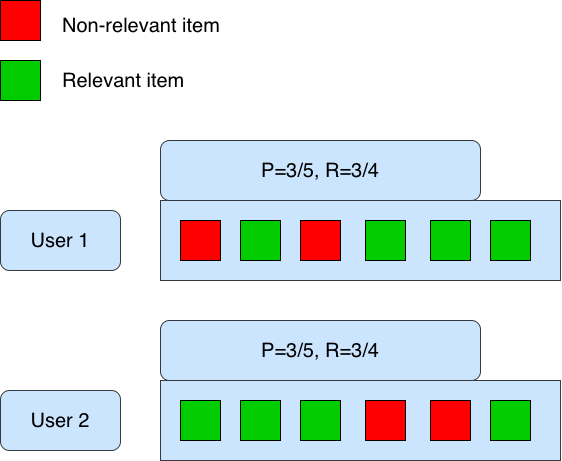
\includegraphics[scale=0.22]{images/precision-recall.png}
   \end{center}
\end{column}
\begin{column}{0.4\textwidth}
    \begin{tcolorbox}[colback=info!5,colframe=info!80,title=]
      \begin{itemize}
      \item Легко интерпретировать
      \item Легко реализовать
      \end{itemize}
    \end{tcolorbox}
    \begin{tcolorbox}[colback=warn!5,colframe=warn!80,title=]
      \begin{itemize}
      \item Нечувствительны к порядку внутри $k$
      \item Не дают общей картины для любого $k$
      \end{itemize}
    \end{tcolorbox}
\end{column}
\end{columns}

\end{frame}

\begin{frame}{Mean Average Precision \cite{MOUSSA}}

\begin{columns}
\begin{column}{0.5\textwidth}
   \begin{center}
		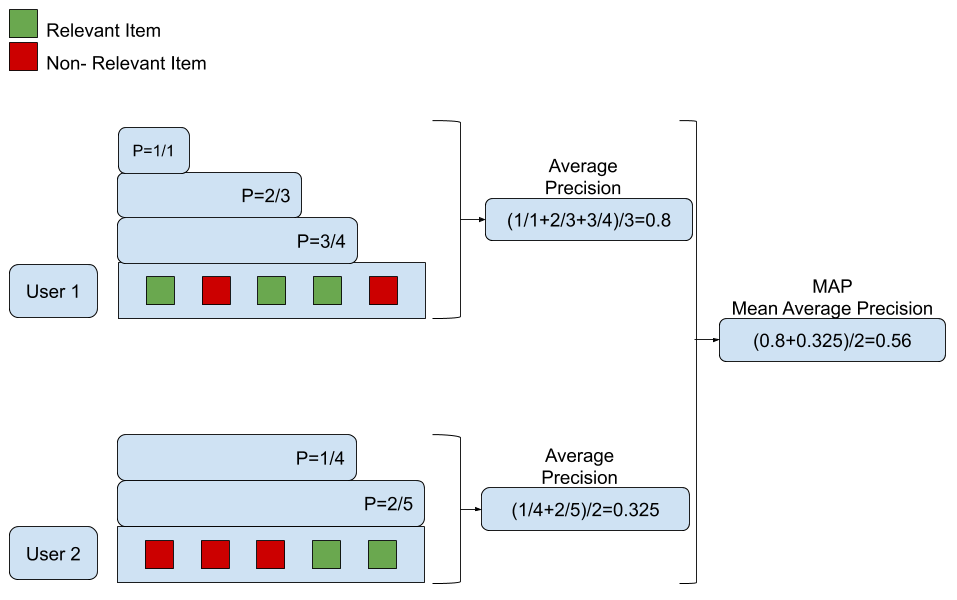
\includegraphics[scale=0.22]{images/map.png}
   \end{center}
\end{column}
\begin{column}{0.4\textwidth}
    \begin{tcolorbox}[colback=info!5,colframe=info!80,title=]
      \begin{itemize}
      \item Дают общую картину качества
      \item Больше внимания айтемам в голове списка
      \end{itemize}
    \end{tcolorbox}
    \begin{tcolorbox}[colback=warn!5,colframe=warn!80,title=]
      \begin{itemize}
      \item Подходит только для бинарного фидбэка
      \end{itemize}
    \end{tcolorbox}
\end{column}
\end{columns}

\end{frame}

\begin{frame}{Area Under Precision-Recall curve}

\begin{columns}
\begin{column}{0.5\textwidth}
   \begin{center}
		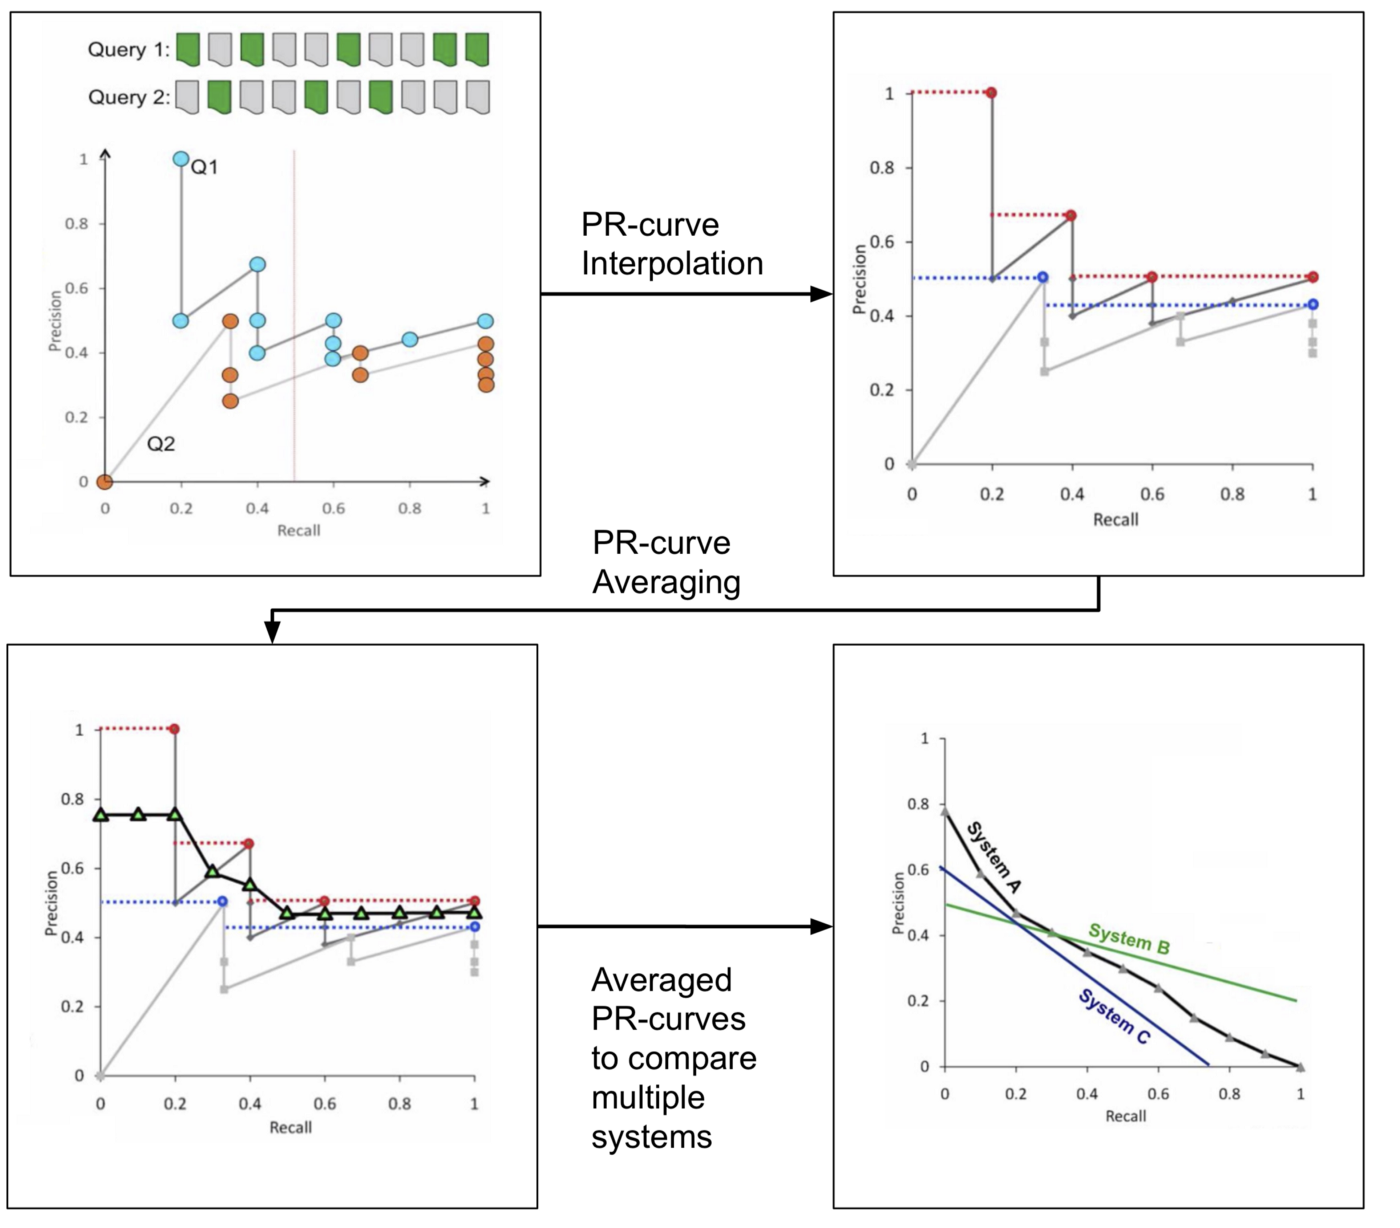
\includegraphics[scale=0.13]{images/auprc.png}
   \end{center}
\end{column}
\begin{column}{0.4\textwidth}
    \begin{tcolorbox}[colback=gray!5,colframe=gray!80,title=]
      Визуальное представление MAP
    \end{tcolorbox}
\end{column}
\end{columns}

\end{frame}

\begin{frame}{MRR}

\begin{columns}
\begin{column}{0.5\textwidth}
   \begin{center}
		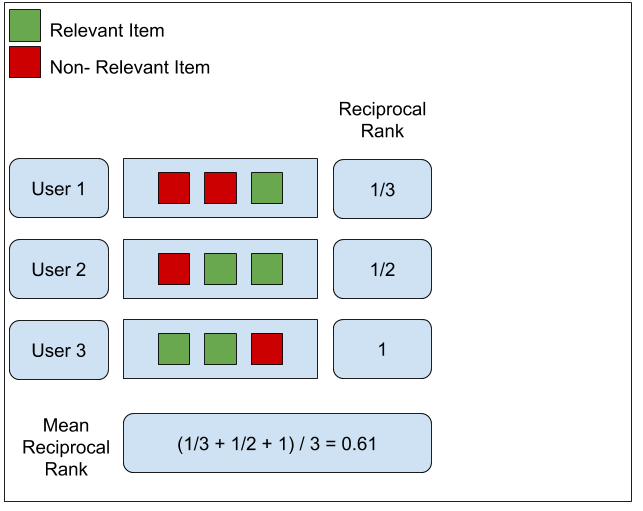
\includegraphics[scale=0.3]{images/mrr.png}
   \end{center}
\end{column}
\begin{column}{0.4\textwidth}
    \begin{tcolorbox}[colback=info!5,colframe=info!80,title=]
      \begin{itemize}
      \item Легко интерпретировать
      \item Легко реализовать
      \item Удобна для задач, где имеет значение первый результат
      \end{itemize}
    \end{tcolorbox}
    \begin{tcolorbox}[colback=warn!5,colframe=warn!80,title=]
      \begin{itemize}
      \item Учитывает только первый результат
      \item Быстро убывает
      \end{itemize}
    \end{tcolorbox}
\end{column}
\end{columns}

\end{frame}

\begin{frame}{[N]DCG}

\begin{columns}
\begin{column}{0.5\textwidth}
   \begin{center}
		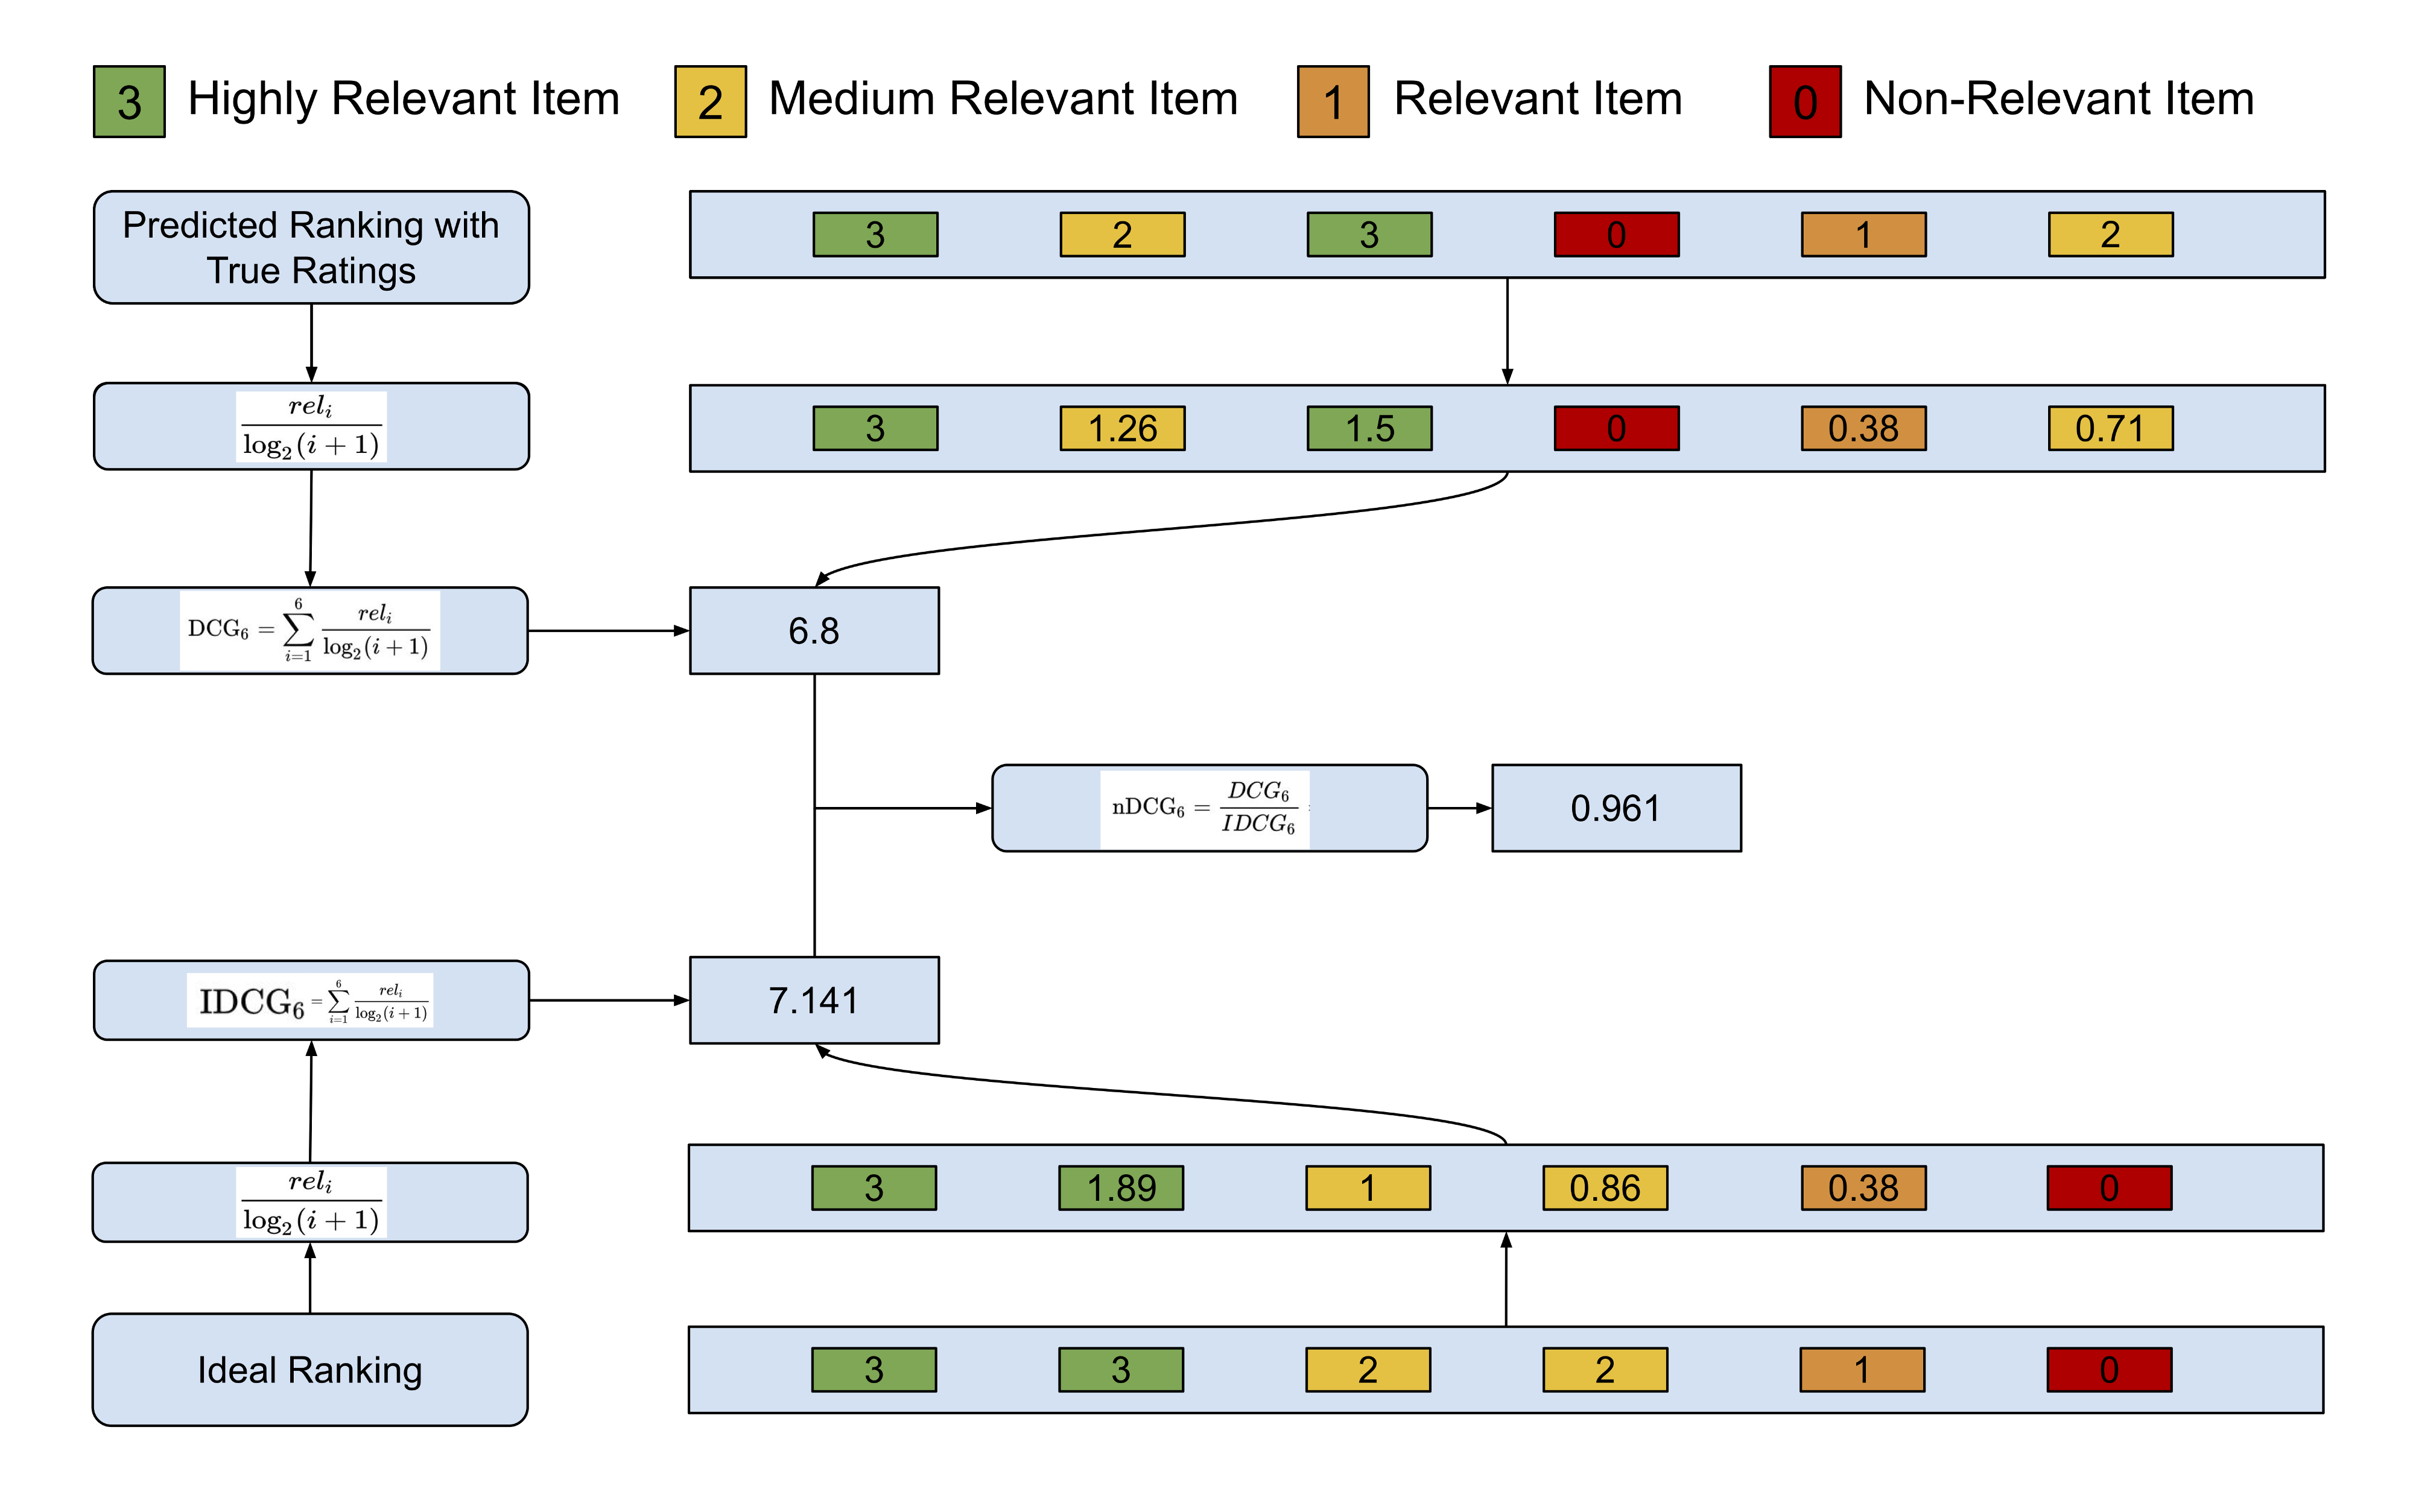
\includegraphics[scale=0.055]{images/ndcg.png}
   \end{center}
\end{column}
\begin{column}{0.4\textwidth}
    \begin{tcolorbox}[colback=info!5,colframe=info!80,title=]
      \begin{itemize}
      \item Учитывает не только бинарный фидбэк
      \item Хорошо учитывает позицию
      \end{itemize}
    \end{tcolorbox}
    \begin{tcolorbox}[colback=warn!5,colframe=warn!80,title=]
      \begin{itemize}
      \item Сложно интерпретировать
      \end{itemize}
    \end{tcolorbox}
\end{column}
\end{columns}

\end{frame}

\begin{frame}{Гайд по выбору метрик Николая Анохина}

\begin{enumerate}
\item Находим метрики релевантности, которые подходят к задаче
\item Выбираем в качестве основной самую интерпретируемую
\item Усложняем метрику, если оказалось, что она не отражает реальность
\end{enumerate}

\end{frame}

\section{Покрытие}

\begin{frame}{Item space coverage}

\begin{tcolorbox}[colback=info!5,colframe=info!80,title=]
Какую долю из всех возможных айтемов умеет рекомендовать сервис?
\end{tcolorbox}

\[
cov = \frac{| I_p |}{| I |}
\]

\[
gini = \frac{1}{| I | - 1} \sum_{j=1}^{| I |}(2 j - | I | - 1) p(I_j)
\]
$p^1(I_j)$ -- частота, с которой пользователи выбирают айтем $I_j$ 

$p^2(I_j)$ -- частота, с которой рекомендер показывает айтем $I_j$ 

Айтемы отсортированы по возрастанию $p(I_j)$ 

\end{frame}

\begin{frame}{User space coverage}

\begin{tcolorbox}[colback=info!5,colframe=info!80,title=]
Доля пользователей, которые могут получить рекомендации
\end{tcolorbox}

\end{frame}

\section{Разнообразие}

\begin{frame}{Разнообразие \cite{KUNAVER}}

\begin{tcolorbox}[colback=info!5,colframe=info!80,title=]
[diversity] Насколько разнообразные айтемы в списке рекомендаций пользователя?
\end{tcolorbox}

\begin{center}
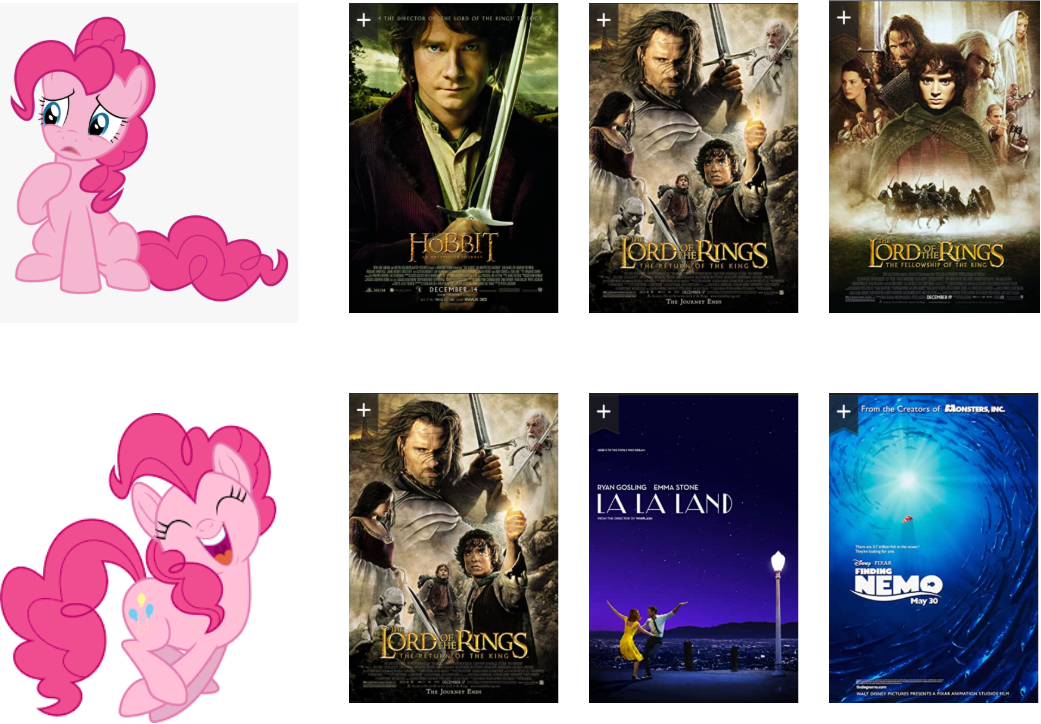
\includegraphics[scale=0.2]{images/diversity.png}
\end{center}

\end{frame}

\begin{frame}

\[
div(u) = \frac{\sum_{i=1}^n \sum_{j=1}^n (1 - similarity(i, j))}{n/2 (n-1)} 
\]

\vfill

\begin{tcolorbox}[colback=gray!5,colframe=gray!80,title=]
With 1\% precision loss, percentage of rec. long-tail items increases from 16 to 32, with 5\% loss perc. increases to 58.
\end{tcolorbox}

\vfill

\begin{tcolorbox}[colback=warn!5,colframe=warn!80,title=]
Метрика сильно зависит от того, как определить сходство
\end{tcolorbox}

\end{frame}

\begin{frame}
Maximal Marginal Relevence \cite{CARBONELL}
\[
MMR = \max_j \left[ \lambda \, similarity(j, U) + (1 - \lambda) \max_{k < j} similarity(k, j) \right]
\]
\end{frame}

\section{Удачность}

\begin{frame}{Удачность}

The term {\bf serendipity} has been recognized as one of the most untranslatable words. 
The first known use of the term was found in a letter by Horace Walpole to Sir Horace Mann on January 28, 1754. 
The author described his discovery by referencing a Persian fairy tale, ``The Three Princes of Serendip''. 
The story described a journey taken by three princes of the country Serendip to explore the world. 
In the letter, Horace Walpole indicated that the princes were ``always making discoveries, by accidents and sagacity, of things which they were not in quest of''. \cite{KOTKOV}

\begin{center}
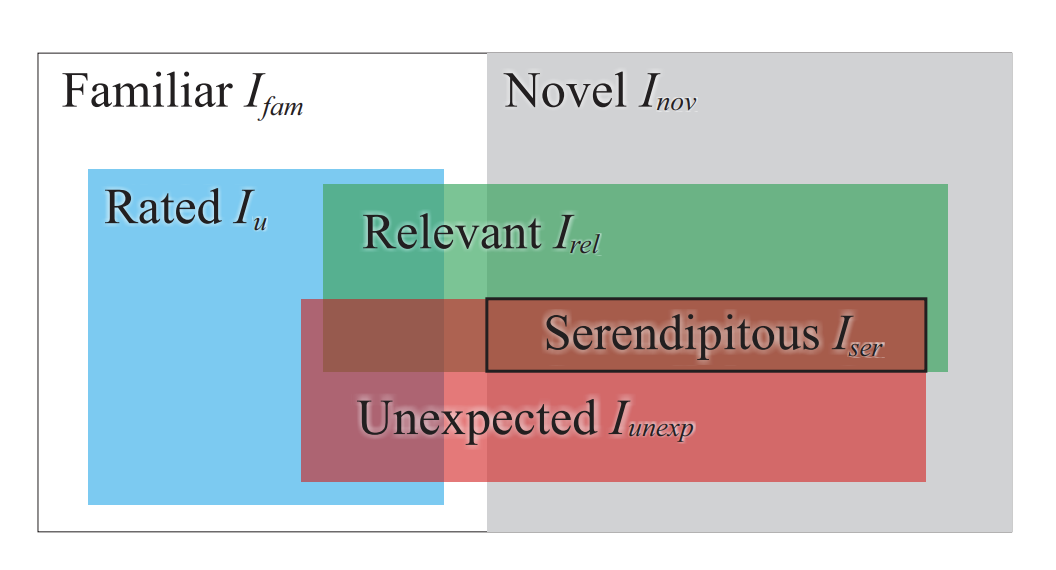
\includegraphics[scale=0.3]{images/serendipity.png}
\end{center}

\end{frame}

\begin{frame}{}
\begin{center}
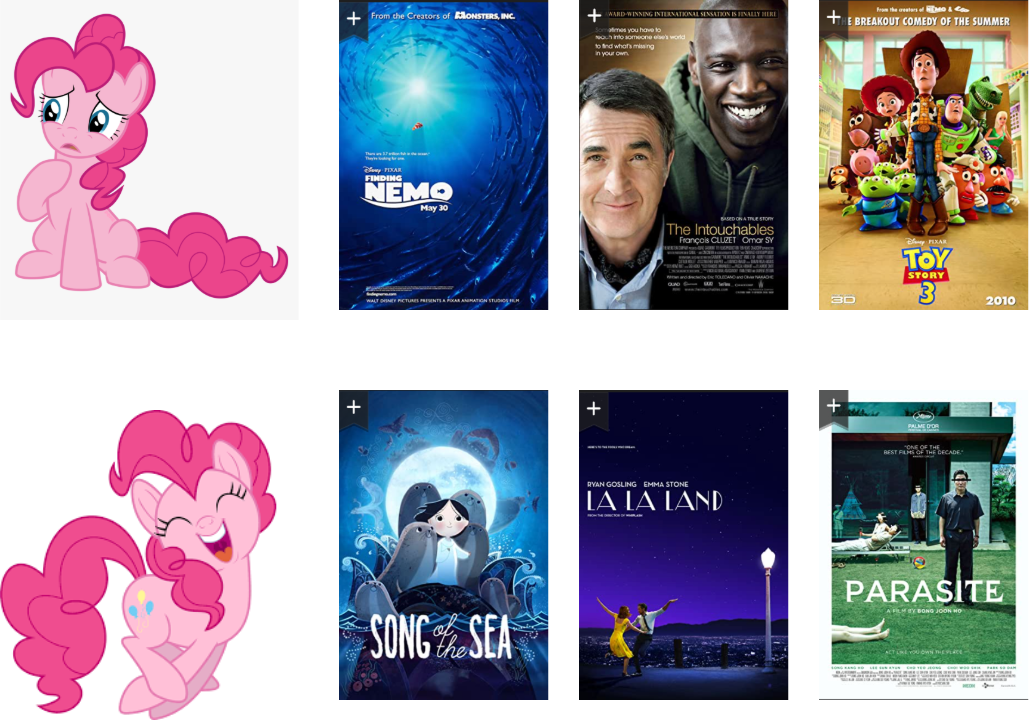
\includegraphics[scale=0.2]{images/serendipity-pony.png}
\end{center}
\end{frame}

\begin{frame}{Новизна}

\begin{tcolorbox}[colback=info!5,colframe=info!80,title=]
[novelty] Насколько айтем неизвестен пользователю?
\end{tcolorbox}

Идея 1: Насколько айтемы близки к айтемам из истории пользователя?
\[
nov^1(u, i) = \min_{j \in I_u} dist(j, i)
\]

Идея 2: Насколько айтемы близки к популярным?
\[
nov^2(u, i) = 1 - \frac{|U_i|}{|U|}
\]

\end{frame}

\begin{frame}{Неожиданность}

\begin{tcolorbox}[colback=info!5,colframe=info!80,title=]
[unexpectedness] Насколько пользователь ожидает увидеть в рекомендациях айтем?
\end{tcolorbox}

\[
nPMI(i, j) = - \log \frac{p(i, j)}{p(i)p(j)} / \log p(i, j)
\]

\[
unexp(u, i) = \max_{j \in I_u} \left( -nPMI(i, j) \right)
\]

\end{frame}

\begin{frame}

\begin{footnotesize}

\begin{center}

\begin{tabular}{l c c c c c}
Цель & rel & cov & div & ser & poll \\
\hline
{\bf Бизнесу} & & & & & \\
\hline
Увеличить продажи & \checked & & & \checked & \\
Продвигать более разнообразные айтемы & & \checked & \checked & \checked & \\
Улучшить пользовательский опыт & \checked & & \checked & \checked & \checked \\
Добиться большей лояльности & & & & & \checked \\
Лучше понимать пользователей & & & & & \checked \\
\hline
{\bf Пользователям} & & & & & \\
\hline
Найти лучший товар & \checked & & & \checked & \checked \\
Найти {\bf все} подходящие товары & \checked & \checked & & & \checked \\
Найти последовательность или набор товаров & & & \checked & & \checked \\
Залипнуть & & & \checked & \checked & \checked \\
Найти рекомендер, которому можно доверять & & & & & \checked \\
Реализовать творческие потребности & & & & & \checked \\
Помочь другим сделать выбор & & & & & \checked \\
\end{tabular}

\end{center}

\end{footnotesize}

\end{frame}

\section{Бейзлайны}

\begin{frame}{}

\begin{tcolorbox}[colback=info!5,colframe=info!80,title=Простые бейзлайны]
\begin{itemize}
\item позволяют определить нижнюю границу качества системы
\item позволяют быстро стартануть
\end{itemize}

\end{tcolorbox}

\vfill

\begin{itemize}%[<+->]
\item Живительный рандом
\item TopPopular
\item Эвристики
\item Редакторская подборка
\end{itemize}

\end{frame}

\section{Итоги}

\begin{frame}{Итоги}

\begin{tcolorbox}[colback=info!5,colframe=info!80,title=]
При выборе подхода к проверке гипотез, нужно иметь в виду компромисс надежности и скорости
\end{tcolorbox}

\begin{tcolorbox}[colback=info!5,colframe=info!80,title=]
Технические метрики отражают разные аспекты рекомендаций: релевантность, разнообразие, удачность
\end{tcolorbox}

\begin{tcolorbox}[colback=info!5,colframe=info!80,title=]
Don't be a hero: не связываемся со сложными алгоритмами, пока не заведем простые бейзлайны
\end{tcolorbox}

\end{frame}

\begin{frame}[allowframebreaks]{Литература}

\bibliographystyle{amsalpha}
\bibliography{references.bib}

\end{frame}

\end{document}
